% =============================================================
%  Project report - Hate speech detection
%  Text (HateXplain) & Multimodal (Hateful Memes / HarMeme)
% =============================================================
\documentclass[11pt,a4paper]{article}

% ---------- Packages ----------
\usepackage[utf8]{inputenc}
\usepackage[T1]{fontenc}
\usepackage[english]{babel}
\usepackage[a4paper,margin=2.3cm]{geometry}
\usepackage{lmodern}
\usepackage{microtype}
\usepackage{graphicx}
\usepackage{booktabs}
\usepackage{array}
\usepackage{multirow}
\usepackage{longtable}
\usepackage{amsmath,amssymb}
\usepackage{xcolor}
\usepackage{hyperref}
\usepackage{listings}
\usepackage{tcolorbox}
\usepackage{caption}
\usepackage{enumitem}
\usepackage{fancyhdr}

\hypersetup{
    colorlinks=true,
    linkcolor=black!70,
    citecolor=black!70,
    urlcolor=blue!60!black,
}

% ---------- Page layout ----------
\pagestyle{fancy}
\fancyhf{}
\fancyhead[L]{\small Hate speech detection --- Text \& Multimodal}
\fancyhead[R]{\small \thepage}
\renewcommand{\headrulewidth}{0.4pt}

% ---------- Result / lesson boxes ----------
\newtcolorbox{lesson}[1][]{%
    colback=blue!4, colframe=blue!50!black,
    fonttitle=\bfseries, title=Lesson learned, #1}
\newtcolorbox{warn}[1][]{%
    colback=red!4, colframe=red!60!black,
    fonttitle=\bfseries, title=Negative result, #1}
\newtcolorbox{insight}[1][]{%
    colback=green!4, colframe=green!40!black,
    fonttitle=\bfseries, title=Key insight, #1}

% ---------- Listings ----------
\lstset{
    basicstyle=\ttfamily\footnotesize,
    breaklines=true,
    frame=single,
    backgroundcolor=\color{gray!8},
    columns=fullflexible,
}

% =============================================================
\title{\textbf{Hate Speech Detection}\\
\large Text and multimodal approaches --- a deep learning project retrospective}
\author{[Author 1] \and [Author 2] \and [Author 3]}
\date{\today}
% =============================================================

\begin{document}
\maketitle

\begin{abstract}
\noindent
This report retraces the full journey of a hate speech detection project carried out
on two complementary fronts: ternary text classification on \textbf{HateXplain}
(hatespeech / normal / offensive), and binary multimodal image+text classification
on \textbf{Hateful Memes} and then \textbf{HarMeme}. We document the initial choices,
the successive iterations, the architectures tested (roberta-base, HateBERT,
CLIP+HateBERT with \emph{late-fusion} then \emph{cross-attention}), the training
techniques (focal loss, label-confidence weighting, partial defrosting), the per
target-group bias analysis, and several owned-up negative results (group-aware
re-weighting, counterfactual augmentation, TTA on memes). A critical image-loading
bug --- discovered late --- invalidated eight multimodal experiments and forced us
to pivot to HarMeme, which is itself one of the most valuable lessons of this project.

\medskip
\noindent\textbf{Final best results:}
\begin{itemize}[leftmargin=*]
    \item HateXplain (3 classes) --- HateBERT + focal loss + warmup + confidence
    weighting: \textbf{test macro-F1 = 0.683}.
    \item HarMeme (binary, multimodal) --- CLIP ViT-B/32 + HateBERT, last 2 layers
    defrosted: \textbf{test AUROC = 0.910}, \textbf{F1 (harmful) = 0.803}.
\end{itemize}
\end{abstract}

\tableofcontents
\vspace{1em}
\hrule

% =============================================================
\section{Introduction}
% =============================================================

Automatic hate speech detection is a societally high-stakes problem, but also an
intrinsically \emph{ambiguous} one: the boundary between aggressive language,
offensive content and actual hate speech is fuzzy, even for trained human
annotators. We tackled this problem from two distinct but complementary angles.

\paragraph{Part 1 --- Text (HateXplain).}
Classifying short social-media posts into three categories: \emph{hatespeech},
\emph{normal} or \emph{offensive}. The core difficulty lies in the middle class:
"offensive" is defined negatively (\emph{neither hateful nor neutral}) and is
therefore structurally hard.

\paragraph{Part 2 --- Multimodal (Hateful Memes, then HarMeme).}
Classifying memes as \emph{hateful} / \emph{not hateful}. A meme combines an image
with a short text overlay; its hateful nature often emerges only from the
\emph{combination} of both modalities (an innocuous caption on an offensive image,
or a dog-whistle phrase on an innocuous image). This is fundamentally a multimodal
problem.

\paragraph{What this report tells.}
Rather than a flat results summary, we chose to retrace the project
\emph{chronologically}: the initial hypotheses, the successive experiments, what
worked, what did not, the bugs we discovered along the way, and the methodological
pivots they forced. We ran 29 documented experiments overall; this report is an
organised synthesis of them.

% =============================================================
\section{Data}
% =============================================================

\subsection{HateXplain (Mathew et al., 2021)}

\begin{itemize}[leftmargin=*]
    \item 15\,383 train / 1\,922 validation / 1\,924 test.
    \item Three classes: \emph{hatespeech} (0), \emph{normal} (1), \emph{offensive} (2).
    Distribution: 36 / 41 / 23\,\%.
    \item Each post is labelled by \textbf{3 independent annotators}; the final
    label is the majority, and a \texttt{label\_confidence} score
    $\in \{0.33, 0.66, 1.0\}$ is provided. This signal is exploited in several
    experiments.
    \item Each annotator also provides token-level \emph{rationales} (which words
    justify the label) and a \emph{target group} (Jewish, Women, African\dots) used
    later for bias analysis.
\end{itemize}

\subsection{Hateful Memes (Facebook / \texttt{limjiayi/hateful\_memes\_expanded})}

\begin{itemize}[leftmargin=*]
    \item 12\,887 / 1\,040 / 3\,000 (train/val/test), binary (58.7\,\% \emph{not\_hateful},
    41.3\,\% \emph{hateful}).
    \item Each example = a meme image + a short caption.
    \item \textbf{Critical issue:} the HuggingFace snapshot only ships the JSONL
    metadata, the images themselves are \emph{not} bundled (licensing). This silent
    omission corrupted all our early multimodal experiments --- see
    section~\ref{sec:bug}.
\end{itemize}

\subsection{HarMeme (Pramanick et al., 2021) --- replacement dataset}

\begin{itemize}[leftmargin=*]
    \item 3\,013 / 177 / 354 (train/val/test). Originally 3 classes
    (\emph{not harmful}, \emph{somewhat harmful}, \emph{very harmful}), binarised
    in our study as \emph{harmful} vs \emph{not\_harmful}.
    \item COVID-themed memes, with text "burned in" the image.
    \item 4$\times$ smaller than Hateful Memes, but the only image-grounded
    multimodal hate/harm benchmark we could obtain locally.
\end{itemize}

% =============================================================
\section{Models, building blocks and techniques}
% =============================================================

\subsection{Backbones}

\begin{description}[leftmargin=*]
    \item[roberta-base.] General-purpose language model pre-trained on broad web
    text. A reasonable baseline.
    \item[GroNLP/hateBERT.] BERT model further pre-trained on the \emph{Reddit
    Abusive Language English corpus} (RAL-E). Domain-specialised on online hate ---
    our hypothesis was that domain pre-training would give a head start.
    \item[openai/clip-vit-base-patch32.] Vision-language encoder pre-trained on
    400M image-text pairs. Its vision encoder yields 50 tokens (CLS + 7$\times$7
    patches) projected to 512-d.
\end{description}

\subsection{Multimodal fusion}

\begin{description}[leftmargin=*]
    \item[Late-fusion via concatenation.] Image CLS (512-d) $\oplus$ text CLS
    (768-d) $\Rightarrow$ MLP. The simplest case; the modalities only meet at the
    output level.
    \item[Bidirectional cross-attention.] $n$ blocks where text tokens attend over
    image patches \emph{and} vice versa, with residuals and FFNs. Expected
    inductive bias for memes: harmfulness emerges from the \emph{interaction}
    between text and image, not from their isolated CLS tokens (VisualBERT, MMBT,
    ViLT).
\end{description}

\subsection{Encoder freezing policies}

\begin{itemize}[leftmargin=*]
    \item \textbf{Fully frozen}: only the head is trained ($\sim$330\,k parameters).
    Cheap, exploits pre-training to the maximum.
    \item \textbf{Defrost the last $N$ blocks} (typ.\ $N=2$): 30\,M to 58\,M
    trainable parameters. \emph{Differential learning rate}: encoder LR = head LR
    $\times 0.1$, to prevent drift.
    \item \textbf{Fully fine-tuned} (HateBERT on HateXplain): everything trains,
    feasible because 15\,k training examples are available.
\end{itemize}

\subsection{Training techniques}

\begin{itemize}[leftmargin=*]
    \item \textbf{Label-confidence weighting}: per-example loss multiplied by
    inter-annotator agreement.
    \item \textbf{Focal loss} ($\gamma=2$): $\mathrm{FL} = (1-p_t)^\gamma \cdot
    \mathrm{CE}$. Focuses training on hard examples and improves calibration (zero
    high-confidence errors consistently observed).
    \item \textbf{Class weights}, inverse-frequency.
    \item \textbf{LR warmup} (6\,\% of steps) \textbf{+ cosine decay}.
    \item \textbf{Gradient clipping} at norm 1.0.
\end{itemize}

\subsection{Inference-time techniques}

\begin{itemize}[leftmargin=*]
    \item \textbf{Threshold tuning}: sweep the threshold on validation to maximise
    F1. Free, sometimes +0.20 F1.
    \item \textbf{Ensembling}: average the softmax outputs of several models, then
    threshold-tune.
    \item \textbf{Test-Time Augmentation (TTA)}: predict on several augmented
    variants (horizontal flip, 5 crops) and average. \emph{Spoiler:} on memes it
    \emph{hurts} (see section~\ref{sec:harmeme}).
\end{itemize}

\subsection{Metrics}

\begin{itemize}[leftmargin=*]
    \item \textbf{Macro-F1} for HateXplain (3 classes): penalises the minority
    "offensive" class.
    \item \textbf{AUROC} for memes (binary): threshold-independent, robust to
    imbalance.
    \item \textbf{F1 (positive class)} at threshold 0.5 and at the tuned threshold,
    on memes.
    \item \textbf{Per-target-group macro-F1} on HateXplain (bias analysis).
\end{itemize}

% =============================================================
\section{Part 1 --- HateXplain: ternary text classification}
% =============================================================

\subsection{Overall strategy}

Our approach was incremental: start from a simple baseline (roberta-base, plain CE,
no tricks), then add the relevant techniques one by one, systematically measuring
their effect on validation macro-F1.

\subsection{Historical first experiments (Exp 1--8)}

These experiments were run on an earlier version of the pipeline. They are kept for
the project's memory but are not directly comparable to the later ones (the
pipeline was refactored: unified preprocessing, JSONL with \texttt{label\_confidence},
cosine scheduler, gradient clipping).

\begin{table}[h]
\centering\small
\caption{Exp 1--8: initial exploration (roberta-base).}
\begin{tabular}{p{0.5cm} p{6.8cm} p{2.3cm} p{2.5cm}}
\toprule
\# & Description & Val macro-F1 & Status \\
\midrule
1 & Historical baseline, max\_length=128 & 0.6874 & historical reference \\
2 & max\_length=256 & 0.6917 & worse on test $\Rightarrow$ rejected \\
3 & Class weights & 0.6747 & rejected \\
4 & Implicit-hate binary (HateXplain vs ImplicitHate) & 0.9842 &
\emph{invalidated}: source confound (Reddit vs Twitter) \\
5 & + token-level rationale supervision ($\alpha=0.5$) & 0.6581 & rejected \\
6 & idem ($\alpha=0.1$) & 0.6544 & rejected \\
7 & Confidence weighting (1\textsuperscript{st} attempt) & --- &
\emph{invalid}: missing field, silent fallback to 1.0 \\
8 & Keep only examples with confidence = 1.0 & 0.6474 &
rejected (losing 50\,\% of data costs more than it yields) \\
\bottomrule
\end{tabular}
\end{table}

\begin{insight}
Several \emph{intuitively reasonable} ideas failed at this stage: widening the
context (2), auxiliary supervision on rationales (5--6), or filtering out ambiguous
examples (8). These shaped our later choices: \textbf{keep all examples, but
soft-down-weight them by annotation confidence}.
\end{insight}

\subsection{Unified pipeline (Exp 9--14)}

After refactoring, we re-ran the key experiments on a clean pipeline.

\begin{table}[h]
\centering\small
\caption{Exp 9--14: unified pipeline.}
\label{tab:hatexplain_main}
\begin{tabular}{p{0.5cm} p{2.2cm} p{5.5cm} c c c}
\toprule
\# & Backbone & Added techniques & Val F1 & Test F1 & Off.\ F1 \\
\midrule
9  & roberta-base & baseline                                & 0.6465 & ---    & ---   \\
10 & roberta-base & + confidence weighting                  & 0.6703 & 0.6631 & 0.518 \\
11 & roberta-base & + focal loss + warmup                   & 0.6560 & 0.6700 & 0.506 \\
12 & roberta-base & + class weights                         & 0.6715 & 0.6625 & 0.533 \\
13 & HateBERT     & focal + warmup + class weights          & 0.6877 & 0.6829 & 0.537 \\
\textbf{14} & \textbf{HateBERT} & \textbf{focal + warmup, no class weights}
              & \textbf{0.6931} & \textbf{0.6827} & \textbf{0.535} \\
\bottomrule
\end{tabular}
\end{table}

\begin{figure}[h]
\centering
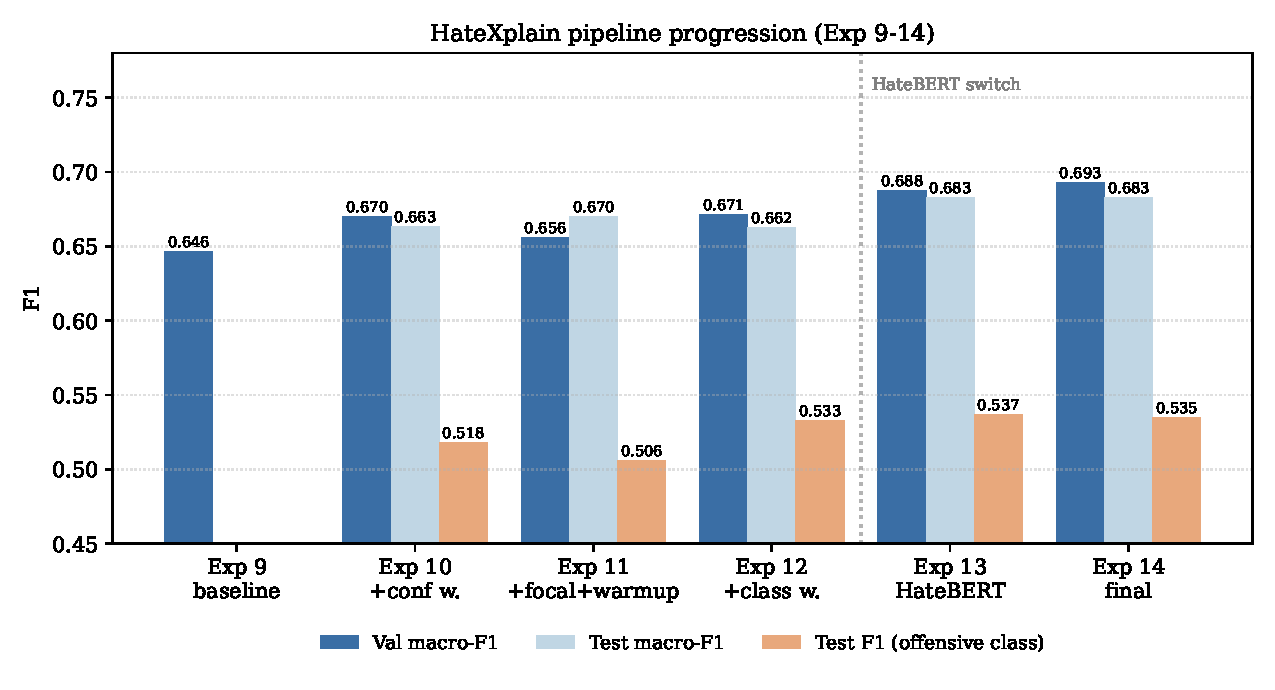
\includegraphics[width=0.95\linewidth]{figures/fig1_hatexplain_progression.pdf}
\caption{Pipeline progression on HateXplain. The HateBERT switch (dotted line)
is the single most impactful change of the whole project. Confidence weighting,
focal loss and class weights together add less than the backbone change alone.}
\label{fig:hatexplain_progression}
\end{figure}

\paragraph{Step-by-step analysis.}
\begin{itemize}[leftmargin=*]
    \item \textbf{Exp 10 (confidence weighting).} +0.024 val F1 vs baseline.
    Down-weighting ambiguous examples beats either throwing them away (Exp 8) or
    using them at full weight.
    \item \textbf{Exp 11 (focal loss + warmup).} Val F1 dips slightly (5-epoch
    overfit) but test F1 goes up and calibration improves: \textbf{zero
    high-confidence errors}, a property that will persist in all subsequent
    focal-trained models.
    \item \textbf{Exp 12 (class weights).} Boosts the \emph{offensive} class
    (0.506 $\to$ 0.533) at the cost of \emph{normal} (0.737 $\to$ 0.699).
    Symmetric trade-off --- discussed below.
    \item \textbf{Exp 13 (HateBERT).} \textbf{Major jump:} +0.016 val F1 vs Exp 12,
    and HateBERT's \emph{epoch 1} already beats the best epoch of any roberta-base
    run. Domain pre-training is by far the single most impactful improvement of
    the whole project.
    \item \textbf{Exp 14 (HateBERT without class weights, ablation).}
    \textbf{Final model.} Removing the class weights does not degrade anything
    (differences $<$0.003): HateBERT already handles imbalance implicitly.
    Simpler is better.
\end{itemize}

\paragraph{Final model details (Exp 14).}
Val macro-F1 = 0.6931; test accuracy = 0.6949; test macro-F1 = 0.6827.
Test confusion matrix:

\begin{center}\small
\begin{tabular}{l|ccc}
\toprule
              & pred\_hate & pred\_norm & pred\_off \\
\midrule
true\_hate    & 478 & 41  & 75  \\
true\_norm    & 55  & 577 & 150 \\
true\_off     & 117 & 149 & 282 \\
\bottomrule
\end{tabular}
\end{center}

\begin{lesson}
\textbf{Domain pre-training matters more than any architectural cleverness.}
Switching roberta-base $\to$ HateBERT yielded +0.123 val F1, more than the
combined effect of confidence weighting, focal loss and class weights together.
\end{lesson}

\paragraph{Why the "offensive" class remains hard.}
The offensive$\leftrightarrow$normal confusion is \emph{symmetric} (149 vs 150) on
every model we trained. This is not a model defect; it is a definitional ambiguity.
"Offensive" is defined as "neither hateful nor normal", and HateXplain reports
33\,\% inter-annotator disagreement on that class.

% =============================================================
\section{Part 1 (cont.) --- Bias analysis and correction attempts}
% =============================================================

\subsection{Motivation}

HateXplain annotates each post with a \emph{target group} (Asian, African, Jewish,
Women\dots). We do not use these labels during training, but we use them post-hoc
to check the fairness of the final model.

\subsection{Per-group results (Exp 14 model)}

\begin{table}[h]
\centering\small
\caption{Macro-F1 per target group on the test set (Exp 14).}
\label{tab:bias_per_group}
\begin{tabular}{l c c c c c c}
\toprule
Group & $N$ & Acc. & Macro-F1 & F1-hate & F1-norm & F1-off \\
\midrule
Asian      & 53  & 0.491 & \textbf{0.467} & 0.619 & 0.474 & 0.308 \\
Hispanic   & 44  & 0.636 & \textbf{0.473} & 0.793 & 0.471 & 0.154 \\
Jewish     & 210 & 0.686 & 0.509 & 0.836 & 0.364 & 0.329 \\
Islam      & 238 & 0.643 & 0.584 & 0.765 & 0.625 & 0.362 \\
African    & 388 & 0.696 & 0.584 & 0.841 & 0.481 & 0.430 \\
Arab       & 90  & 0.711 & 0.593 & 0.852 & 0.483 & 0.444 \\
Caucasian  & 114 & 0.632 & 0.617 & 0.667 & 0.698 & 0.485 \\
Homosexual & 223 & 0.610 & 0.619 & 0.643 & 0.661 & 0.551 \\
Refugee    & 113 & 0.664 & 0.647 & 0.634 & 0.746 & 0.560 \\
Women      & 233 & 0.670 & 0.664 & 0.640 & 0.696 & 0.657 \\
Other      & 244 & 0.705 & \textbf{0.690} & 0.667 & 0.663 & 0.741 \\
\midrule
\multicolumn{4}{l}{\textbf{Gap (best $-$ worst) = 0.223}} & & & \\
\bottomrule
\end{tabular}
\end{table}

\begin{figure}[h]
\centering
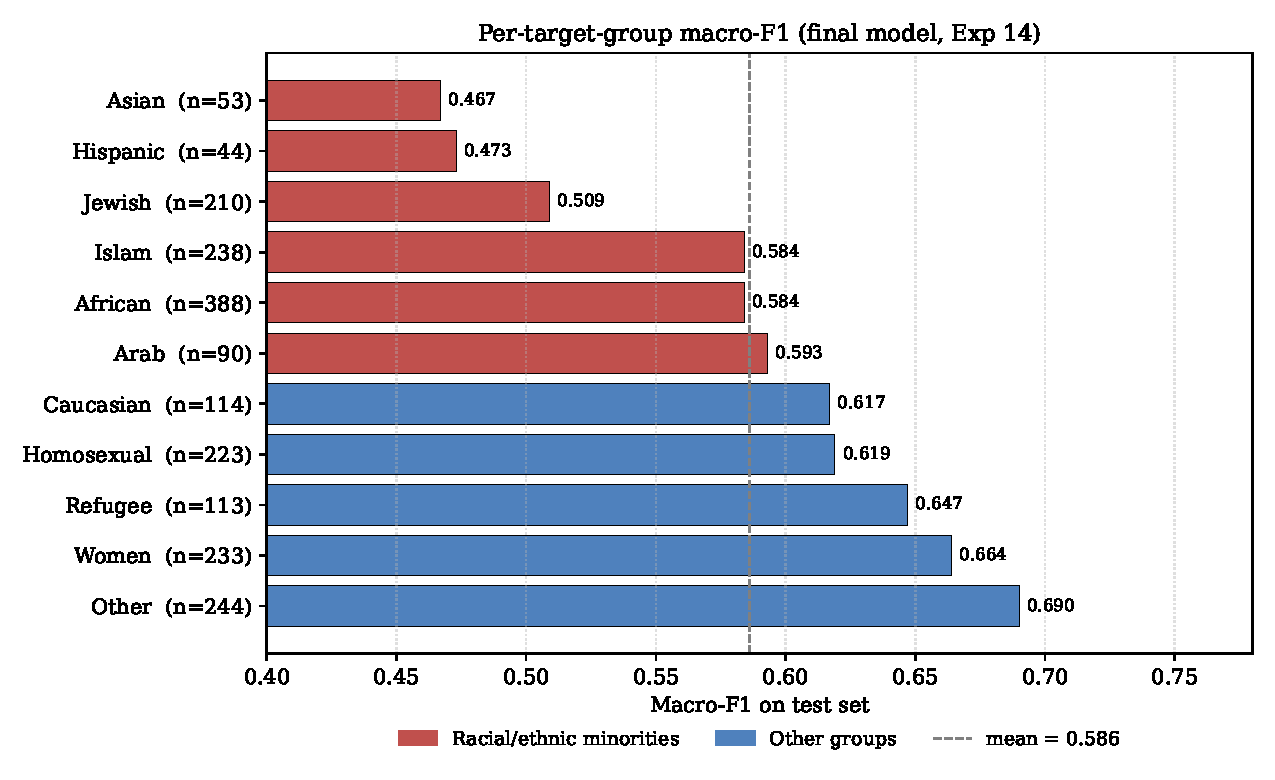
\includegraphics[width=0.95\linewidth]{figures/fig2_bias_per_group.pdf}
\caption{Macro-F1 per target group on the test set, sorted ascending. The six
worst-performing groups (red) are all racial/ethnic minorities; the four best
(blue) are not. The gap between Asian (0.467) and Other (0.690) is 0.223.}
\label{fig:bias_per_group}
\end{figure}

\subsection{Diagnosis: a spurious shortcut}

The six worst-performing groups are all racial/ethnic minorities. For each of them
the F1 on the \emph{hate} class is high (0.76--0.85) but the F1 on \emph{normal} or
\emph{offensive} collapses (as low as 0.15 for Hispanic). Explanation: those groups
predominantly appear in hateful contexts in training (Jewish: 68\,\% hate;
African: 60\,\%; Arab: 59\,\%). The model has learned a shortcut "mention of group
$\Rightarrow$ hate", which works when the post is indeed hateful but fails badly
otherwise.

The bias also runs the other way: "Caucasian" mostly appears in \emph{normal}
posts (53\,\%), so the model has a \emph{low} F1-hate on that group.

\subsection{Attempt 1 --- (Group, class) re-weighting (Exp 18, 19)}

We computed, for each example, a weight inversely proportional to the frequency of
its (group, class) pair, multiplied with the confidence weighting.

\begin{warn}
Both versions (Exp 18 with a normalisation bug, Exp 19 with the fix) \textbf{hurt
overall performance by $\sim$3.5\,pp} \emph{without} reducing the inter-group gap.
Worse: the gap \emph{grew} to 0.264 in Exp 18. Diagnosis: the smallest groups
(Asian: $\sim$50 train examples, Hispanic: $\sim$44) lack data; up-weighting them
does not create signal, only noise.
\end{warn}

\subsection{Attempt 2 --- Counterfactual augmentation (Exp 28, 29)}

Inspired by Liang et al.\ (2020), we generated, for each post identified as
targeting a group, copies in which the group is swapped:

\begin{lstlisting}[language={}]
Original : "kikes are responsible for the bad economy"  (hate, Jewish)
CF #1    : "blacks are responsible for the bad economy"  (hate, African)
CF #2    : "asians are responsible for the bad economy"  (hate, Asian)
\end{lstlisting}

Two policies tested: (a) augment only hate/offensive posts; (b) augment all
classes to keep balance.

\begin{table}[h]
\centering\small
\caption{Counterfactual augmentation: results.}
\begin{tabular}{l c c c c c}
\toprule
\# & CF policy & Train rows & Val F1 & Test F1 & Bias gap \\
\midrule
14 & none                          & 15\,383 & 0.693 & 0.683 & \textbf{0.223} \\
28 & hate + offensive only         & 27\,463 & 0.678 & 0.666 & 0.306 (worse) \\
29 & all classes (balanced)        & 31\,425 & 0.665 & 0.640 & 0.265 (worse) \\
\bottomrule
\end{tabular}
\end{table}

\begin{figure}[h]
\centering
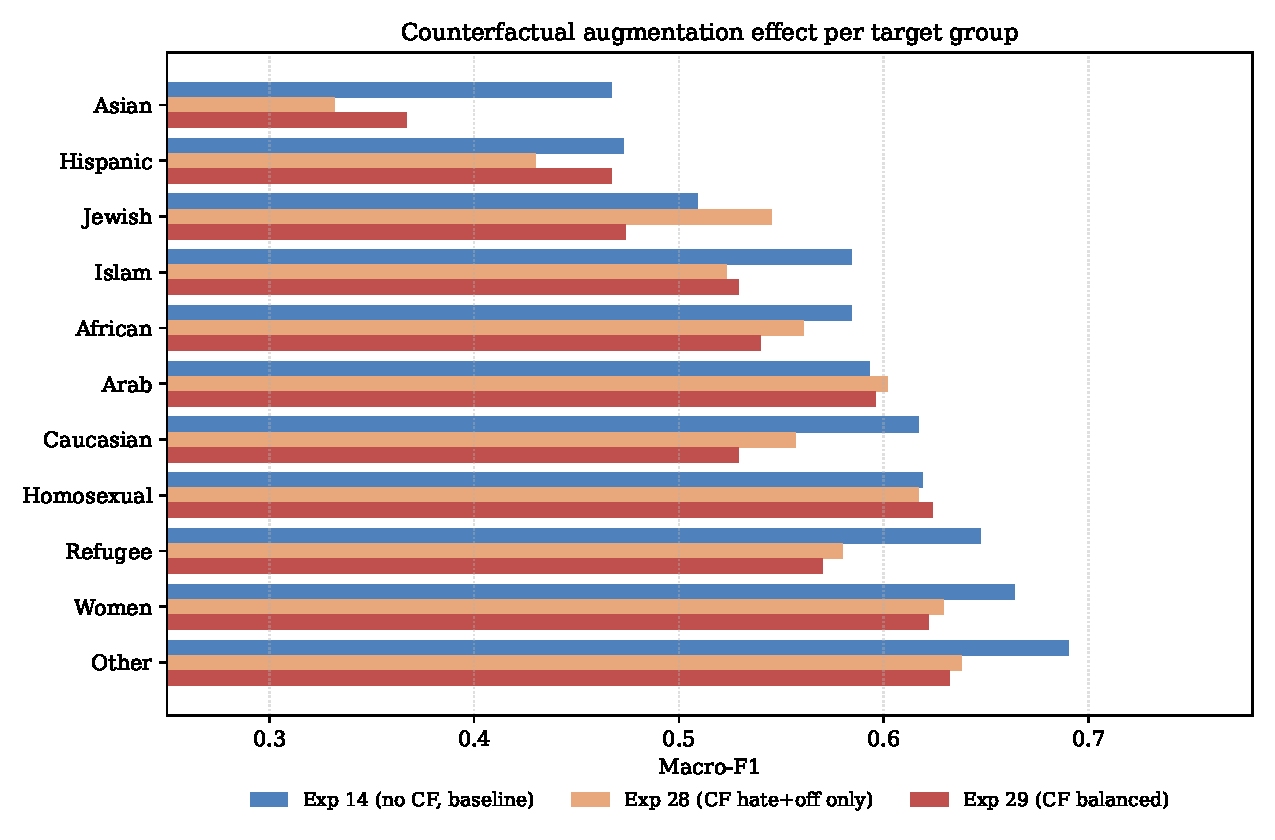
\includegraphics[width=0.95\linewidth]{figures/fig6_cf_augment.pdf}
\caption{Per-group macro-F1 for the baseline (Exp 14) and both CF policies
(Exp 28, 29). Almost every group regresses under augmentation, including the
previously best one (\emph{Other}). The two smallest groups (Asian, Hispanic)
are the most damaged by Exp 28.}
\label{fig:cf_augment}
\end{figure}

\begin{warn}
Both versions \textbf{worsened} the bias gap. Three hypotheses:
(1) HateBERT's priors (RAL-E) on group-hate co-occurrences are deeper than the
$\sim$1\,000 synthetic examples we added;
(2) the single-token lexical detector misses $\sim$33\,\% of multi-word group
references;
(3) substitutions inject label noise ("kikes" $\to$ "muslims" in an idiom no
longer makes sense).
\end{warn}

\begin{lesson}
\textbf{Bias in hate speech detection is resistant to surface-level corrections.}
Both our approaches (group re-weighting, lexical CF augmentation) failed,
consistent with the literature (Davidson et al.\ 2019, Sap et al.\ 2019). The
remaining paths --- not explored for lack of time --- are LLM-based generative
augmentation, adversarial debiasing (gradient reversal on the group), or, most
likely, more balanced data collection per group.
\end{lesson}

% =============================================================
\section{Part 2 --- Hateful Memes: multimodal classification}
% =============================================================

\subsection{Initial architecture: CLIP + HateBERT, frozen late-fusion}

We first wanted a clean baseline with frozen encoders and a simple fusion:

\begin{center}\small\ttfamily
Image \(\to\) CLIP ViT-B/32 (frozen) \(\to\) 512-d \\
                                       \(\oplus\) concat \(\to\) MLP \(\to\) logits \\
Text  \(\to\) HateBERT (frozen) \(\to\) 768-d
\end{center}

\textbf{Choices and rationale.}
\begin{itemize}[leftmargin=*]
    \item Frozen encoders: fast training (5 min/epoch), no catastrophic forgetting.
    \item CLIP as the image encoder: pre-trained on image-text pairs, already
    semantically aligned with language.
    \item HateBERT as the text encoder: the best hate backbone identified in Part 1.
    \item Late-fusion: a minimalist baseline before trying anything fancier.
\end{itemize}

\subsection{Modality ablation (Exp 15--17)}

To check that multimodality actually helps, we compared three \emph{strictly
identical} architectures (a disabled modality is replaced by a zero tensor).

\begin{table}[h]
\centering\small
\caption{Modality ablation (Exp 15--17). \textbf{$\Rightarrow$ results later
invalidated by the \emph{grey-placeholder bug}, see section~\ref{sec:bug}.}}
\begin{tabular}{l c c c c}
\toprule
Condition & Trainable params & Test Acc. & F1 (hateful) & AUROC \\
\midrule
15 -- Text-only (HateBERT)        & 197\,k & 0.590 & 0.361 & 0.610 \\
16 -- Image-only (CLIP)           & 132\,k & 0.619 & 0.425 & 0.671 \\
\textbf{17 -- Multimodal}         & \textbf{328\,k} & \textbf{0.658} & \textbf{0.494} & \textbf{0.718} \\
\bottomrule
\end{tabular}
\end{table}

\begin{figure}[h]
\centering
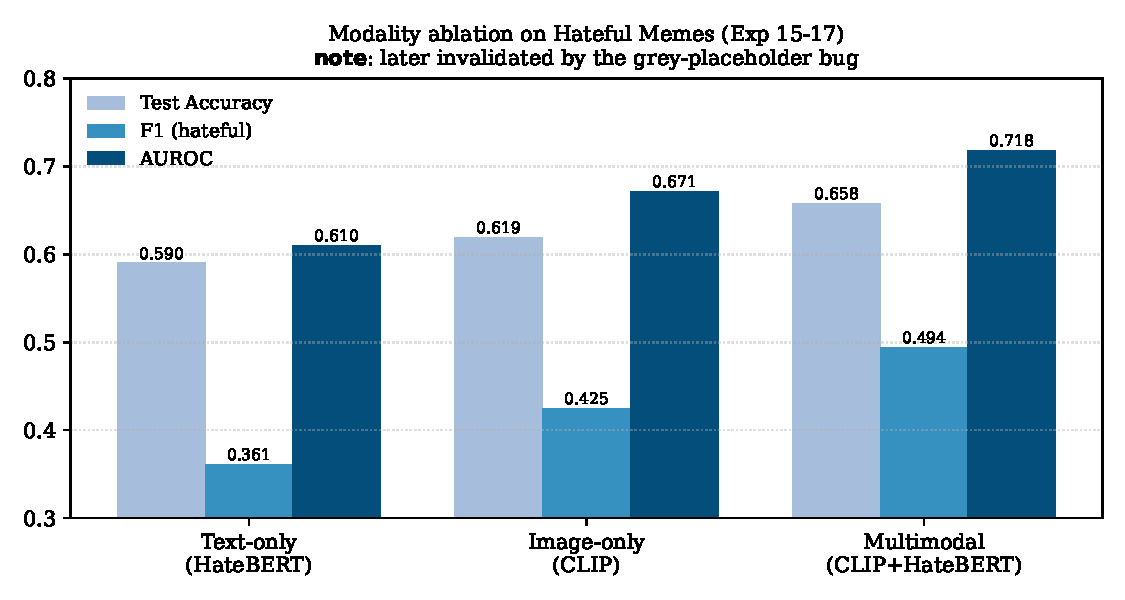
\includegraphics[width=0.85\linewidth]{figures/fig3_memes_modality.pdf}
\caption{Modality ablation on Hateful Memes (Exp 15--17). \emph{What we
believed at the time.} These numbers were later invalidated by the
grey-placeholder bug (section~\ref{sec:bug}): the visual branch was fed a
uniformly grey tensor.}
\label{fig:memes_modality}
\end{figure}

At that point of the project, we concluded:
\begin{itemize}[leftmargin=*]
    \item \emph{Image $>$ Text} for memes (captions are often deliberately
    innocuous).
    \item \emph{Fusion $>$ Image alone}, gain of +0.047 AUROC.
    \item Training only 0.13\,\% of 261\,M parameters is enough with frozen
    encoders.
\end{itemize}

\subsection{Capacity-scaling attempts (Exp 20--23)}

The baseline plateaued at AUROC 0.718 and missed 60\,\% of hateful memes
(recall 0.404). Natural question: can we improve by \emph{defrosting} some encoder
layers, or by replacing concatenation with \emph{cross-attention}?

\begin{table}[h]
\centering\small
\caption{Capacity scaling on Hateful Memes (same code/machine/seed). \textbf{$\Rightarrow$
also affected by the image bug.}}
\begin{tabular}{l l c c c c}
\toprule
\# & Architecture & Trainable & Val AUC & Test AUC & F1 tuned \\
\midrule
22 (control) & Frozen late-fusion (re-run of Exp 17, same machine) & 328\,k & 0.6106 & 0.6058 & 0.596 \\
20 & Defrost late-fusion (last 2 layers)              & 29.7\,M & 0.6141 & 0.6176 & 0.599 \\
\textbf{21} & \textbf{Cross-attention + defrost}      & \textbf{57.9\,M} & \textbf{0.6304} & \textbf{0.6249} & 0.597 \\
\bottomrule
\end{tabular}
\end{table}

\paragraph{\emph{Provisional} conclusions (at this point in the project).}
\begin{enumerate}[leftmargin=*]
    \item Cross-attention beats the frozen baseline on AUC (+0.019 test).
    \item Pure defrost is not enough on its own: it has to be combined with an
    architecture that can exploit the extra capacity.
    \item Threshold tuning gives a massive boost (+0.20 F1): the models are
    severely miscalibrated, with optimal thresholds in 0.06--0.17.
\end{enumerate}

\noindent That last point (an anomalously skewed calibration) should have raised a
red flag. \emph{It did, but too late.}

% =============================================================
\section{The pivot: a critical bug and the switch to HarMeme}
\label{sec:bug}
% =============================================================

\subsection{The "grey-placeholder" bug}

Checking how sensitive the model was to a \texttt{torch.flip} of the input image,
we noticed that \emph{the forward returned identical logits}. Investigation: the
\texttt{HatefulMemesDataset} class used a silent fallback that returned a uniformly
\textbf{grey image (RGB=128)} whenever an image file was missing. And the HuggingFace
snapshot \texttt{limjiayi/hateful\_memes\_expanded} only ships JSONL metadata: the
images do not exist on disk.

\begin{warn}
\textbf{All multimodal experiments 15--23 were trained with a uniformly grey image
as visual input.} The "image-only" result in Exp 16 (AUROC 0.671) is wrong; the
"image $>$ text" conclusion does not hold; the defrost-vs-cross-attention
comparison on Hateful Memes was in fact a comparison of three head architectures
fed information-less visual features. The bug went undetected for 8 experiments.
\end{warn}

\paragraph{Why it did not look absurd at first.} The models had plausible AUROC
values (0.60--0.72) because the \emph{text} branch worked, and the head learned a
text-only model disguised as multimodal. The only real diagnostic was the optimal
threshold (0.06--0.17), well off 0.5, a symptom of missing informative signal.

\paragraph{Fixes applied.}
\begin{enumerate}[leftmargin=*]
    \item \texttt{dataset\_memes.py} now accepts an explicit \texttt{local\_img\_dir}
    and \textbf{raises \texttt{FileNotFoundError}} at init time if files are
    missing (\texttt{strict\_images: true}).
    \item Mandatory sanity check before any multimodal training:
\begin{lstlisting}[language={}]
flipped = torch.flip(batch["pixel_values"], dims=[3])
out1 = model(pixel_values=batch["pixel_values"], ...)
out2 = model(pixel_values=flipped, ...)
assert not torch.allclose(out1["logits"], out2["logits"]), \
    "Flip-invariant model -> images likely grey placeholders!"
\end{lstlisting}
\end{enumerate}

\paragraph{Original Hateful Memes = unrecoverable.} DrivenData has archived the
competition, and all available HF copies only ship metadata. We therefore
\textbf{pivoted to HarMeme} (COVID memes with real local images provided by the
user), the only image-grounded harmfulness benchmark we could obtain.

\subsection{HarMeme: architecture re-evaluation (Exp 24--27)}
\label{sec:harmeme}

\begin{table}[h]
\centering\small
\caption{HarMeme: comparable runs (same machine/seed/versions).}
\label{tab:harmeme}
\begin{tabular}{l l c c c c c}
\toprule
\# & Architecture & Trainable & Test AUC & F1@0.5 & F1 tuned & Tuned thr \\
\midrule
24 & Frozen late-fusion (baseline)            & 328\,k    & 0.8766 & 0.7510 & 0.7538 & 0.510 \\
\textbf{25} & \textbf{Defrost late-fusion (last 2)} & 29.7\,M  & \textbf{0.9101} & \textbf{0.8045} & \textbf{0.8033} & 0.700 \\
26 & Cross-attention + defrost                & 57.9\,M   & 0.8829 & 0.6905 & 0.7715 & 0.890 \\
27a & Uniform ensemble (24+25+26)             & ---       & 0.8991 & 0.7560 & 0.8000 & 0.730 \\
27b & Ensemble + TTA (flip + 5 crops)         & ---       & 0.8909 & 0.7361 & 0.7764 & 0.700 \\
\bottomrule
\end{tabular}
\end{table}

\begin{figure}[h]
\centering
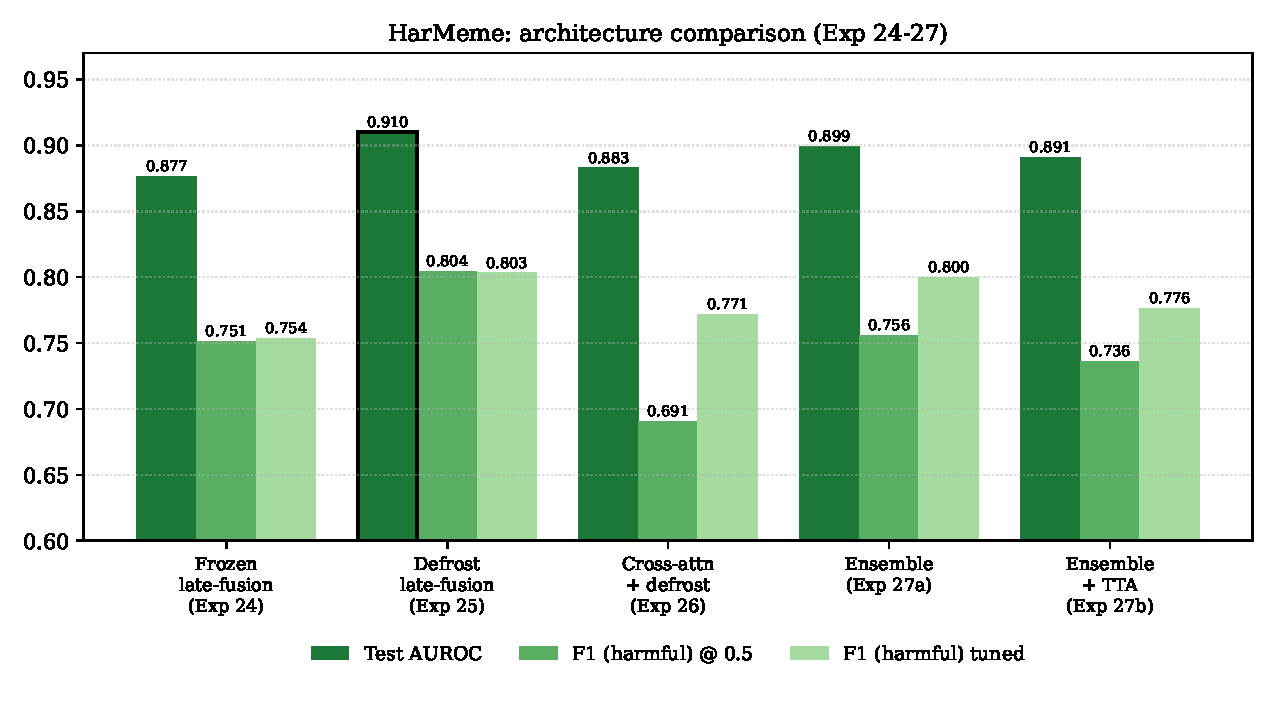
\includegraphics[width=0.95\linewidth]{figures/fig4_harmeme_archs.pdf}
\caption{HarMeme architecture comparison. Defrost (Exp 25, highlighted) wins
clearly on every metric. Cross-attention adds 28M random fusion parameters that
fail to stabilise on 3\,013 examples. The ensemble does not improve over its
strongest member; TTA actively degrades the result.}
\label{fig:harmeme_archs}
\end{figure}

\begin{figure}[h]
\centering
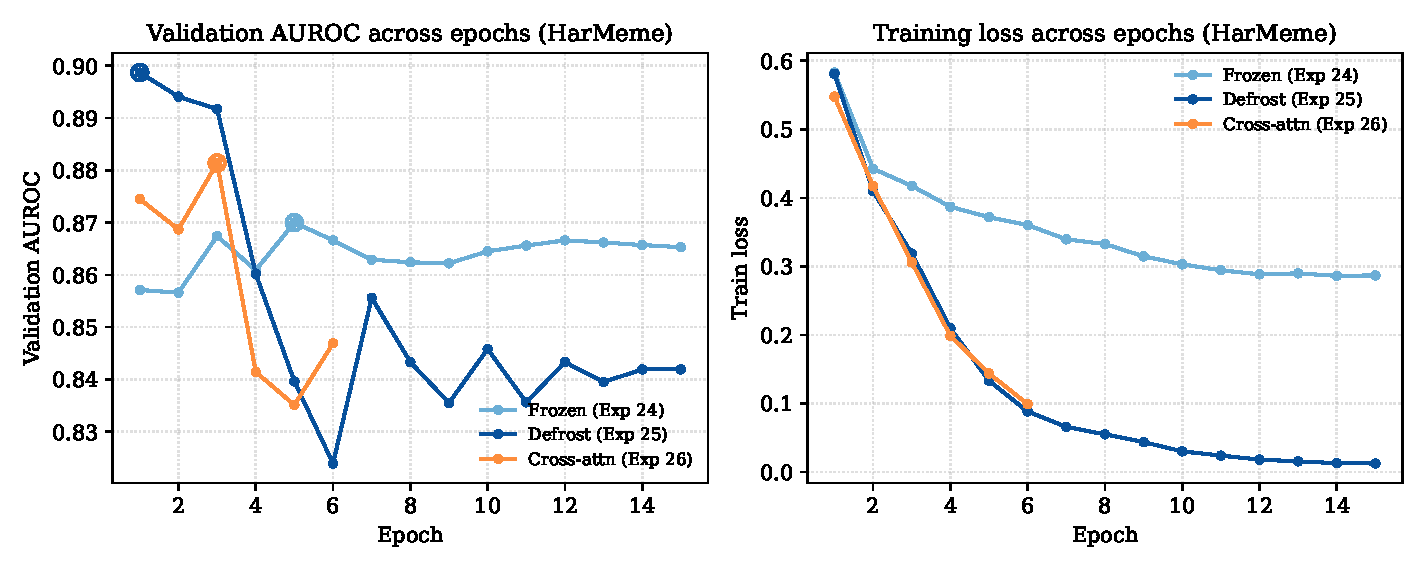
\includegraphics[width=0.99\linewidth]{figures/fig5_harmeme_training.pdf}
\caption{Training dynamics on HarMeme. \emph{Left:} validation AUROC across
epochs --- defrost (Exp 25) peaks at epoch 1 (circled) and slowly decays as the
model overfits the small training set; the frozen baseline keeps improving
slowly; cross-attention peaks at epoch 3 then decays.
\emph{Right:} train loss --- defrost reaches near-memorisation (0.013)
by epoch 15, while the frozen head cannot overfit because of its limited
capacity.}
\label{fig:harmeme_training}
\end{figure}

\paragraph{What changed once real images were provided.}
\begin{enumerate}[leftmargin=*]
    \item \textbf{Defrost becomes the best strategy}, +0.034 AUC vs frozen. This
    is exactly the \emph{opposite} of what we found on broken-Hateful-Memes. With a
    real visual signal, the last 2 CLIP/HateBERT layers have something to refine.
    \item Cross-attention \emph{no longer} beats defrost. With only 3\,013
    examples, its 28\,M randomly-initialised parameters do not stabilise.
    \item Models are \textbf{well-calibrated}: optimal thresholds 0.51 (frozen)
    and 0.70 (defrost), both close to 0.5. Threshold tuning now gains only a few
    hundredths, whereas it gained +0.20 on the broken models.
    \item The ensemble \emph{does not} beat the best member alone: averaging a
    strong model with two weaker ones drags the prediction down.
    \item \textbf{TTA hurts} (--0.024 F1): horizontal flip and 5-crop mangle the
    burned-in text of the meme, which is precisely the information to exploit.
\end{enumerate}

\paragraph{Final model details (Exp 25).}
Val AUROC = 0.8987 (reached at epoch 1), test AUROC = 0.9101, F1 (harmful)
@ 0.5 = 0.8045 (precision 0.753, recall 0.863).

\begin{center}\small
\begin{tabular}{l|cc}
\toprule
              & pred\_not & pred\_harm \\
\midrule
true\_not     & 195       & 35  \\
true\_harm    & 17        & 107 \\
\bottomrule
\end{tabular}
\end{center}

\begin{figure}[h]
\centering
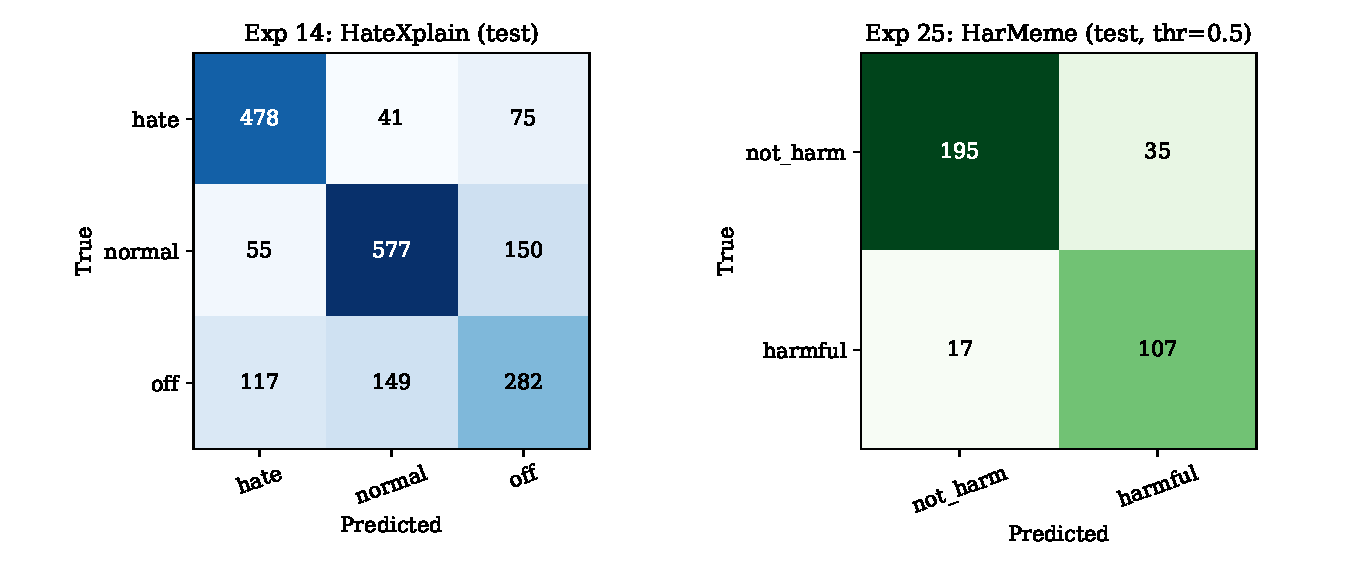
\includegraphics[width=0.95\linewidth]{figures/fig7_confusion.pdf}
\caption{Confusion matrices of the two final models.
\emph{Left:} HateXplain (Exp 14) --- note the symmetric normal$\leftrightarrow$offensive
confusion (149 vs 150), characteristic of a label-ambiguity boundary.
\emph{Right:} HarMeme (Exp 25) at threshold 0.5 --- very few false negatives
(17/124 harmful memes missed).}
\label{fig:confusion}
\end{figure}

\begin{insight}
Defrost peaks at epoch 1 on a 3\,013-example dataset: pre-training already does
80\,\% of the work, one pass over the data is enough to adapt the representations,
later epochs just over-fit.
\end{insight}

% =============================================================
\section{Synthesis: what the project taught us}
% =============================================================

\subsection{Positive lessons}

\begin{enumerate}[leftmargin=*]
    \item \textbf{Domain pre-training beats architectural cleverness.}
    HateBERT vs roberta-base: +0.123 val F1 with zero architecture change. No
    other intervention in the project (focal, class weights, cross-attention,
    group weights, CF) had a comparable effect.
    \item \textbf{Confidence weighting is a free win} on multi-annotator datasets
    (+0.024 val F1, robust).
    \item \textbf{Focal loss improves calibration}: zero high-confidence errors on
    \emph{every} focal-trained model, regardless of macro-F1.
    \item \textbf{Threshold tuning is free \emph{when} the model is miscalibrated}
    (+0.20 F1 on the broken models, $<$0.01 on the well-calibrated ones). Always
    check the optimal threshold before claiming anything.
    \item \textbf{On a \emph{real} multimodal dataset} (HarMeme), defrosting the
    last 2 layers with an encoder LR 10$\times$ smaller than the head is the most
    effective strategy --- better than cross-attention, which requires more data.
\end{enumerate}

\subsection{Owned-up negative results}

\begin{enumerate}[leftmargin=*]
    \item \textbf{Class weights} helped with roberta-base, but were useless with
    HateBERT. Domain representations already encode the class boundary.
    \item \textbf{Group-aware loss weighting} (Exp 18, 19): overall performance
    drops by 3.5\,pp, bias gap \emph{grows}. Re-weighting cannot create missing
    data.
    \item \textbf{Counterfactual augmentation} (Exp 28, 29): both policies
    worsened the bias gap. Single-token substitutions are too shallow against the
    priors of an encoder massively pre-trained on hateful text.
    \item \textbf{TTA on memes}: --0.024 F1. Invariance assumption violated:
    the text is \emph{inside} the image.
    \item \textbf{Uniform ensembling}: drags the best model down when other
    members are weaker.
\end{enumerate}

\subsection{The worst bug in the project, and what it taught us}

The grey-placeholder bug invalidated 8 experiments. It also nearly survived into
the final report. Two takeaways:

\begin{enumerate}[leftmargin=*]
    \item \textbf{Data loaders should fail loudly, not silently.} An explicit
    \texttt{FileNotFoundError} at init would have saved weeks.
    \item \textbf{Sanity checks should target model \emph{outputs}, not just
    inputs.} A "does a horizontal flip change the logits?" test would have caught
    the bug in 30 seconds.
\end{enumerate}

% =============================================================
\section{Selected final models}
% =============================================================

\begin{table}[h]
\centering\small
\caption{Final selected models.}
\begin{tabular}{l l l l}
\toprule
Task & Model & Val metric & Test metric \\
\midrule
HateXplain (3-class) & HateBERT + focal + warmup + conf.\ weighting
& macro-F1 = 0.693 & macro-F1 = 0.683 \\
HarMeme (binary, multimodal) & CLIP + HateBERT, last 2 layers defrosted
& AUROC = 0.899 & AUROC = 0.910 \\
& & & F1 tuned = 0.803 \\
\bottomrule
\end{tabular}
\end{table}

% =============================================================
\section{Limitations and future work}
% =============================================================

\begin{itemize}[leftmargin=*]
    \item \textbf{"Offensive" class is structurally hard} (F1 $\approx$ 0.535).
    The confusion with "normal" is symmetric: this is partly an annotation problem,
    not just a modelling one. Possible avenue: redefine the label space, or
    explicitly leverage the per-annotator distribution (probabilistic model over
    the triplet).
    \item \textbf{Original Hateful Memes is not locally reproducible.} HarMeme
    (3\,013 train, 354 test) is smaller and topically narrower (COVID), so absolute
    numbers cannot be compared to the Hateful Memes literature.
    \item \textbf{Inter-group bias remains unresolved.} Neither re-weighting nor
    naive CF worked. Promising untested directions: adversarial debiasing
    (Zhang et al.\ 2018), LLM-based generative augmentation, or targeted data
    collection for under-represented groups.
    \item \textbf{No per-modality ablation on HarMeme.} The test set is only 354
    examples; the contrast would not be statistically meaningful. The
    "image $>$ text" conclusion from Hateful Memes was invalidated, and we do
    not replace it for lack of a clean re-run.
    \item \textbf{No comparison against an end-to-end vision-language model}
    (BLIP, LLaVA, Flamingo). State of the art on Hateful Memes is above 0.85
    AUROC; our 0.91 on HarMeme is competitive but on a different benchmark.
\end{itemize}

% =============================================================
\section{Conclusion}
% =============================================================

This project covered a wide slice of the deep learning pipeline applied to a
socially loaded problem: backbone choice, multimodal fusion, label-ambiguity
handling, inter-group bias, pipeline debugging. The final results (macro-F1 =
0.683 on HateXplain; AUROC = 0.910 on HarMeme) are solid, but what is probably
most useful for the future is the set of negative results and the bug-forced
\emph{pivot}: they delineate what does not work and why, which is as valuable as
what does.

% =============================================================
\section*{Work distribution (to adapt)}
% =============================================================

\noindent
\textbf{[Author 1]} --- [Part 1 HateXplain, bias analysis, \dots].\\
\textbf{[Author 2]} --- [Part 2 multimodal, CLIP+HateBERT pipeline, \dots].\\
\textbf{[Author 3]} --- [Counterfactual augmentation, ensemble \& TTA, writing, \dots].

% =============================================================
\section*{References}
% =============================================================

\begin{enumerate}[leftmargin=*]
    \item Mathew, B. et al. (2021). \emph{HateXplain: A Benchmark Dataset for
    Explainable Hate Speech Detection}. AAAI.
    \item Caselli, T. et al. (2021). \emph{HateBERT: Retraining BERT for Abusive
    Language Detection in English}. WOAH.
    \item Radford, A. et al. (2021). \emph{Learning Transferable Visual Models From
    Natural Language Supervision (CLIP)}. ICML.
    \item Lin, T.-Y. et al. (2017). \emph{Focal Loss for Dense Object Detection}.
    ICCV.
    \item Kiela, D. et al. (2020). \emph{The Hateful Memes Challenge: Detecting
    Hate Speech in Multimodal Memes}. NeurIPS.
    \item Pramanick, S. et al. (2021). \emph{Detecting Harmful Memes and Their
    Targets}. ACL Findings.
    \item Davidson, T. et al. (2019). \emph{Racial Bias in Hate Speech and Abusive
    Language Detection Datasets}. ACL WS.
    \item Sap, M. et al. (2019). \emph{The Risk of Racial Bias in Hate Speech
    Detection}. ACL.
    \item Liang, P.~P. et al. (2020). \emph{Towards Debiasing Sentence
    Representations}. ACL.
    \item Zhang, B.~H. et al. (2018). \emph{Mitigating Unwanted Biases with
    Adversarial Learning}. AIES.
\end{enumerate}

\end{document}
ch and Abusive
    Language Detection Datasets}. ACL WS.
    \item Sap, M. et al. (2019). \emph{The Risk of Racial Bias in Hate Speech
    Detection}. ACL.
    \item Liang, P.~P. et al. (2020). \emph{Towards Debiasing Sentence
    Representations}. ACL.
    \item Zhang, B.~H. et al. (2018). \emph{Mitigating Unwanted Biases with
    Adversarial Learning}. AIES.
\end{enumerate}

\end{document}
